\chapter{Opis projektnog zadatka}
		
		
		
		Tema našeg projektnog rada je izrada web aplikacije \textit{"BytePit"} koja omogućuje korisnicima sudjelovanje u programerskim natjecanjima i provjeru riješenih zadataka. Ideja je da naša stranica ima sve potrebno za obavljanje natjecanja poput registracije korisnika, uključivanje u natjecanje, pribavljanje zadataka, vrjednovanje priloženih rješenja, prikaz dosadašnjih uspjeha natjecatelja i još mnogo toga.
	
		Neregistrirani korisnik može se registrirati definirajući registrira li se kao \textbf{voditelj} ili \textbf{natjecatelj}
		Za registraciju korisnika potrebno je  unjeti \begin{packed_item}
			\item korisničko ime
			\item fotografiju
			\item lozinku
			\item ime
			\item prezime
			\item email adresu
		\end{packed_item}
		Upješnost registracije potvrđuje se preko email adrdese dok dodatno voditelja potvrđuje i administrator.
		
		\textbf{\textit{Neregistrirani korisnik}} na web stranici može vidjeti kalendar s natjecanjima kojima je moguće pristupiti te pregledati zadatke na stranici. Također, omogućen mu je uvid u profile natjecatelja i voditelja. Svi registrirani korisnici automatski nasljeđuju sve ove mogućnosti koje neregistrirani korisnici imaju.
		
	    \textbf{\textit{Natjecatelj}} prisustuje natjecanjima te dobiva uvid u svoje rezultate. U svrhu pripreme za spomenuta natjecanja, na stranici su dostupni zadatci za vježbu te je dostupna opcija virtualnog natjecanja.
	    
	    \textbf{\textit{Voditelj}} ima veće ovlasti od natjecatelja. U njegovim rukama leži zadatak učitavanja novih zadataka na web aplikaciju te organizacija natjecanja. Kada voditelj izradi natjecanje, ono postaje vidljivo u kalendaru dostupnom natjecateljima. Dakle, zadatak voditelja je odrediti težinu natjecateljskog ispita, broj zadataka i dostupno vrijeme za rješavanje istih te postavljanje termina ispita. Ukoliko želi, voditelj može učitati sličicu pehara.  
	    
	    \textbf{\textit{Administrator}} ima, naravno, najviše ovlasti među navedenima. On može vidjeti popis svih registriranih korisnika zajedno s njihovim osobnim podatcima te im on onda dodjeljuje prava i po potrebi mijenja osobne podatke. Također, može uređivati sve zadatke i natjecanja koja su voditelji postavili na aplikaciju. Administratorova dužnost je ne zloupotrebljavati osobne podatke korisnika, što je i kažnjivo zakonom.\\
	    
	    Na profilu natjecatelja prikazana je statistička obrada njegovih dosadašnjih uspjeha. Stoga mu na profilu možemo vidjeti koliko je zadataka uspješno riješio a koliko ih je pokušavao riješiti te koliko je natjecanja osvojio. Za svako osvojeno natjecanje, na profilu će mu biti prikazana po jedna slikica pehara.
	    Profil voditelja prikazuje popis zadataka koje je on učitao te natjecanja koje je on organizirao. \\
	
		\noindent{\Large {Provedba natjecanja}}\\
		
		\noindent{\Large {Virtualno natjecanje}}\\
		
		\noindent{\Large {Slične str,korisnost,upotreba str.}}\\
		\eject
		
		
		
		\section{Primjeri u \LaTeX u}
		
		\textit{Ovo potpoglavlje izbrisati.}\\

		U nastavku se nalaze različiti primjeri kako koristiti osnovne funkcionalnosti \LaTeX a koje su potrebne za izradu dokumentacije. Za dodatnu pomoć obratiti se asistentu na projektu ili potražiti upute na sljedećim web sjedištima:
		\begin{itemize}
			\item Upute za izradu diplomskog rada u \LaTeX u - \url{https://www.fer.unizg.hr/_download/repository/LaTeX-upute.pdf}
			\item \LaTeX\ projekt - \url{https://www.latex-project.org/help/}
			\item StackExchange za Tex - \url{https://tex.stackexchange.com/}\\
		
		\end{itemize} 	


		
		\noindent \underbar{podcrtani tekst}, \textbf{podebljani tekst}, 	\textit{nagnuti tekst}\\
		\noindent \normalsize primjer \large primjer \Large primjer \LARGE {primjer} \huge {primjer} \Huge primjer \normalsize
				
		\begin{packed_item}
			
			\item  primjer
			\item  primjer
			\item  primjer
			\item[] \begin{packed_enum}
				\item primjer
				\item[] \begin{packed_enum}
					\item[1.a] primjer
					\item[b] primjer
				\end{packed_enum}
				\item primjer
			\end{packed_enum}
			
		\end{packed_item}
		
		\noindent primjer url-a: \url{https://www.fer.unizg.hr/predmet/proinz/projekt}
		
		\noindent posebni znakovi: \# \$ \% \& \{ \} \_ 
		$|$ $<$ $>$ 
		\^{} 
		\~{} 
		$\backslash$ 
		
		
		\begin{longtblr}[
			label=none,
			entry=none
			]{
				width = \textwidth,
				colspec={|X[8,l]|X[8, l]|X[16, l]|}, 
				rowhead = 1,
			} %definicija širine tablice, širine stupaca, poravnanje i broja redaka naslova tablice
			\hline \SetCell[c=3]{c}{\textbf{naslov unutar tablice}}	 \\ \hline[3pt]
			\SetCell{LightGreen}IDKorisnik & INT	&  	Lorem ipsum dolor sit amet, consectetur adipiscing elit, sed do eiusmod  	\\ \hline
			korisnickoIme	& VARCHAR &   	\\ \hline 
			email & VARCHAR &   \\ \hline 
			ime & VARCHAR	&  		\\ \hline 
			\SetCell{LightBlue} primjer	& VARCHAR &   	\\ \hline 
		\end{longtblr}
		

		\begin{longtblr}[
				caption = {Naslov s referencom izvan tablice},
				entry = {Short Caption},
			]{
				width = \textwidth, 
				colspec = {|X[8,l]|X[8,l]|X[16,l]|}, 
				rowhead = 1,
			}
			\hline
			\SetCell{LightGreen}IDKorisnik & INT	&  	Lorem ipsum dolor sit amet, consectetur adipiscing elit, sed do eiusmod  	\\ \hline
			korisnickoIme	& VARCHAR &   	\\ \hline 
			email & VARCHAR &   \\ \hline 
			ime & VARCHAR	&  		\\ \hline 
			\SetCell{LightBlue} primjer	& VARCHAR &   	\\ \hline 
		\end{longtblr}
	


		
		
		%unos slike
		\begin{figure}[H]
			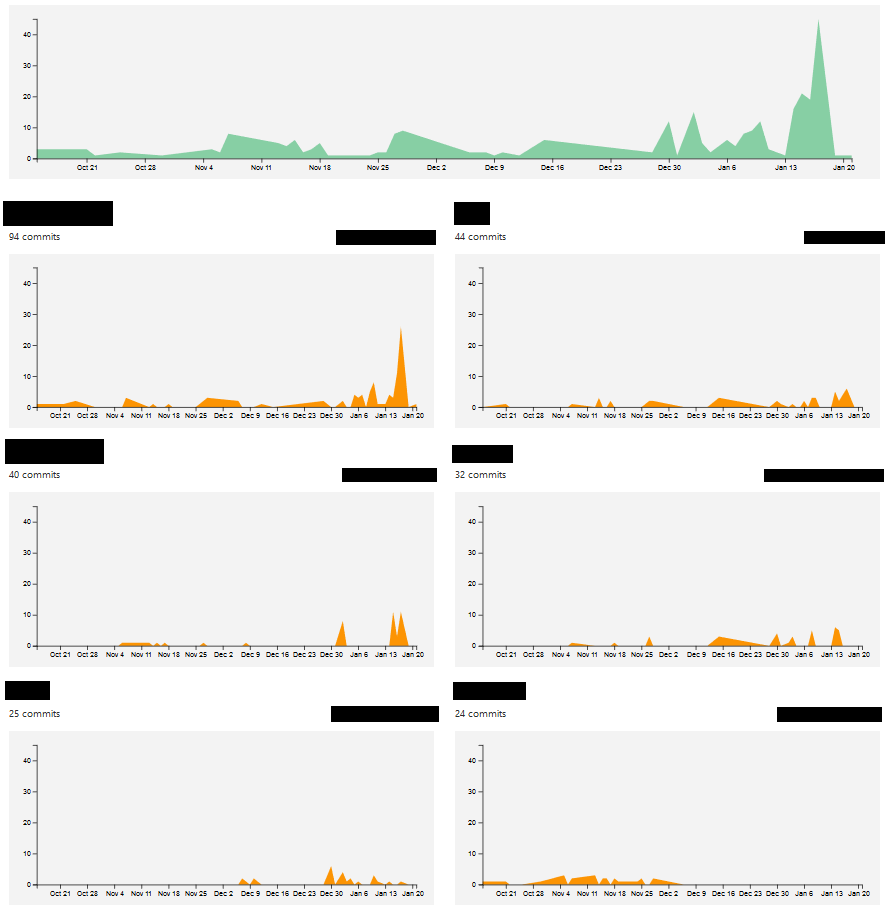
\includegraphics[scale=0.4]{slike/aktivnost.PNG} %veličina slike u odnosu na originalnu datoteku i pozicija slike
			\centering
			\caption{Primjer slike s potpisom}
			\label{fig:promjene}
		\end{figure}
		
		\begin{figure}[H]
			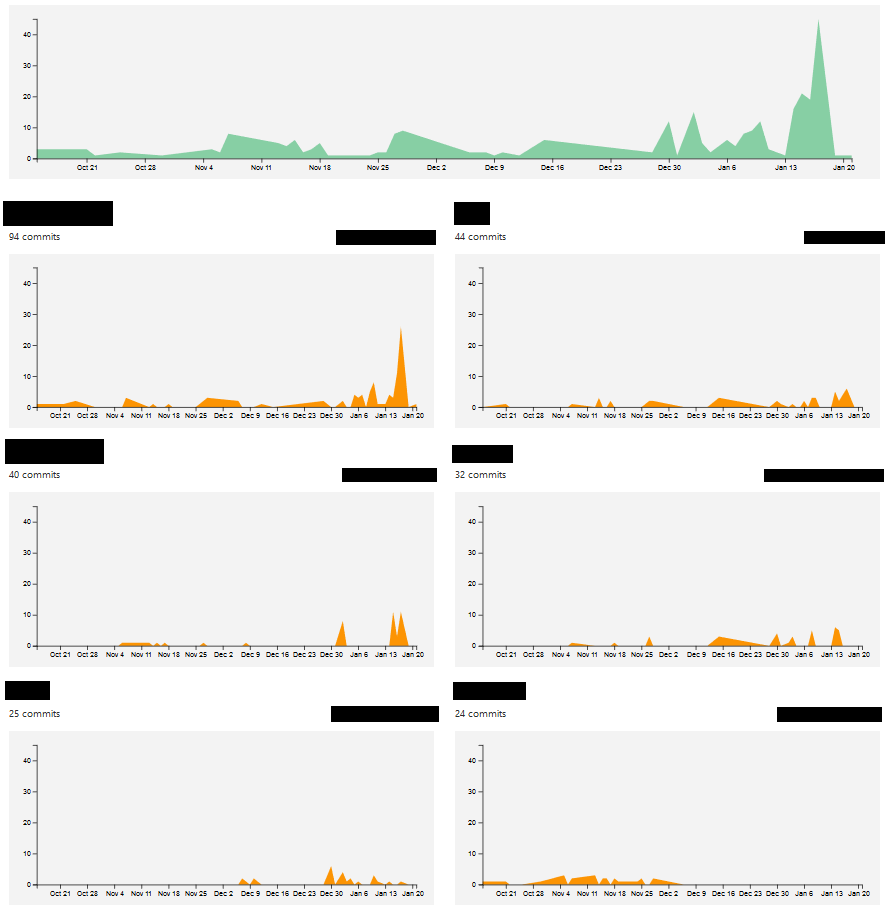
\includegraphics[width=\textwidth]{slike/aktivnost.PNG} %veličina u odnosu na širinu linije
			\caption{Primjer slike s potpisom 2}
			\label{fig:promjene2} %label mora biti drugaciji za svaku sliku
		\end{figure}
		
		Referenciranje slike \ref{fig:promjene2} u tekstu.
		
		\eject
		
	